\documentclass[10pt,a4paper]{article}
\usepackage[russian]{babel}
\usepackage{graphicx}
\usepackage[utf8]{inputenc}
\usepackage[left=1.5cm,right=1.5cm,top=1.5cm]{geometry}
%\pagenumbering{gobble}% Remove page numbers (and reset to 1)

\begin{document}

\begin{center}{\bfseries\Large\scshape Результаты проверки конспектов}\\
Кружок сёги пятого класса ЛНМО, урок 19.11.2015
\end{center}

\noindent
Не секрет, что многие учащиеся не очень хорошо умеют вести конспекты.
Об этом, в частности, шла речь на родительском собрании перед каникулами.
Чтобы помочь детям, родителям и преподавателям, на занятии по сёги 
19 ноября 2015 года были собраны конспекты на проверку.

\medskip\noindent
Поскольку оценка за конспекты за первую четверть уже была выставлена, оценивалось только
качество ведения конспекта на последнем занятии.

\medskip\noindent
На уроке был рассказан дебют \emph{йокофу/йокофудори}
(<<боковая пешка>>/<<взятие боковой пешки>>) с двумя вариантами развития после 11 хода.
На доске была записана следующая информация (и ожидалось, что хотя бы она будет отражена в конспекте):
\begin{itemize}
\setlength{\parskip}{-1ex}\relax
\item[---] название дебюта;
\item[---] последовательность ходов до развилки;
%\item[---] комментарии к ходам;
\item[---] диаграмма позиции в точке развилки;
\item[---] два варианта развития (быстрая и медленная атака) с комментариями;
\item[---] ловушка во втором варианте
\end{itemize}

\noindent
Мною оценивались: наличие тетради, полнота отражения материала и качество записи (точность и читаемость).
В результате проверки были выставлены следующие оценки за конспекты. Эти оценки не пойдут в ведомость и
поставлены лишь как ориентир качества ведения конспекта. Однако далее, как и в конце первой четверти, 
оценка за конспект будет учитываться в итоговой оценке.

\bigskip
\begin{tabular}{llp{10cm}}
Фамилия Имя (Отчество) & Оценка & Комментарий \\
\hline
Андрианов Илья & $4-$ & Отсутствует запись второго варианта\\
Ващенков Алексей & 3 & Неправильная диаграмма, варианты свалены в кучу без комментариев\\
Веселкова Варвара & $4-$ & Неправильное название дебюта, неполный вариант, нет комментариев\\
Данилова Любовь & 2 & Тетрадь есть, дебют назван неточно (<<дебют какой-то>>), неполная запись ходов, 
нет комментариев, отсутствуют варианты и диаграмма\\
Добренко & 2 & Отсутствует тетрадь, запись на рваном листочке, неправильное название дебюта, без комментариев\\
Драган Арина & 2 & Тетрадь есть, конспект урока состоит из заголовка\\
Дунямалиев Руслан & 2 & Тетрадь есть, полностью отсутствует запись урока\\
Иванов Антон Олегович & $3+$ & Последовательность ходов приведена без пояснений, 
                            разобраться в этом, не зная дебюта, невозможно.\\
Каракозов Павел & $4+$ & Отсутствует диаграмма, однако запись аккуратная и понятная\\
Назаров Сергей & $4-$ & Пропущен ход в одном из вариантов, отсутствуют комментарии\\
Нематова Рената & $5-$ & Не совсем правильная диаграмма, но чёткая запись комментариев и вариантов\\
Семёнов Тян-Шанский Егор & $4-$ & Недорисованная диаграмма, отсутствует часть комментариев\\
Сухомлин Фёдор & $5-$ & Ошибки в диаграмме, но чёткая запись вариантов и комментариев, включая некоторые, сделанные
                        только на словах\\
Толкачёв Кирилл & 2 & Отсутствует тетрадь, неправильная и неполная запись\\
Травин Александр & 3 & Неправильное название, отстутствуют комментарии, однако ходы указаны\\
Без имени  & 3 & Отсутствует запись вариантов и комментарии, неверная диаграмма\\
Без имени (папка)  & 4 & Нет комментариев\\
Без имени  & 4 & Диаграммы отсутствуют, но аккуратная чёткая запись\\
\hline
\end{tabular}

\bigskip\noindent
Все остальные ученики конспект на проверку не предоставили; возможно, он у них отсутствует.

\medskip\noindent
Итого: 9 человек из 27 (один отсутствовал на занятии) ведут конспект на 4- или лучше.

\medskip\noindent
С одной стороны, я отмечаю прогресс: раньше конспектов обычно просто не было.
Однако, ещё предстоит очень много работы. 
Я написал этот документ ради обратной
связи, далее приведён пример нормального, на мой взгляд, конспекта
за этот урок. Будет очень хорошо разобрать этот пример родителям вместе с ребёнком, 
чтобы отличия его конспекта от данного стали очевидны.

%\medskip\noindent
%К сожалению, ученики часто надеются, что они закроют глаза и <<этот кошмар>> 
%рассосётся сам. Давайте их в этом разубедим. Со своей стороны я готов и дальше
%периодически брать конспекты на проверку.

\begin{center}\bfseries Пример записи в конспекте, отражающей все ключевые пункты занятия:

\bigskip
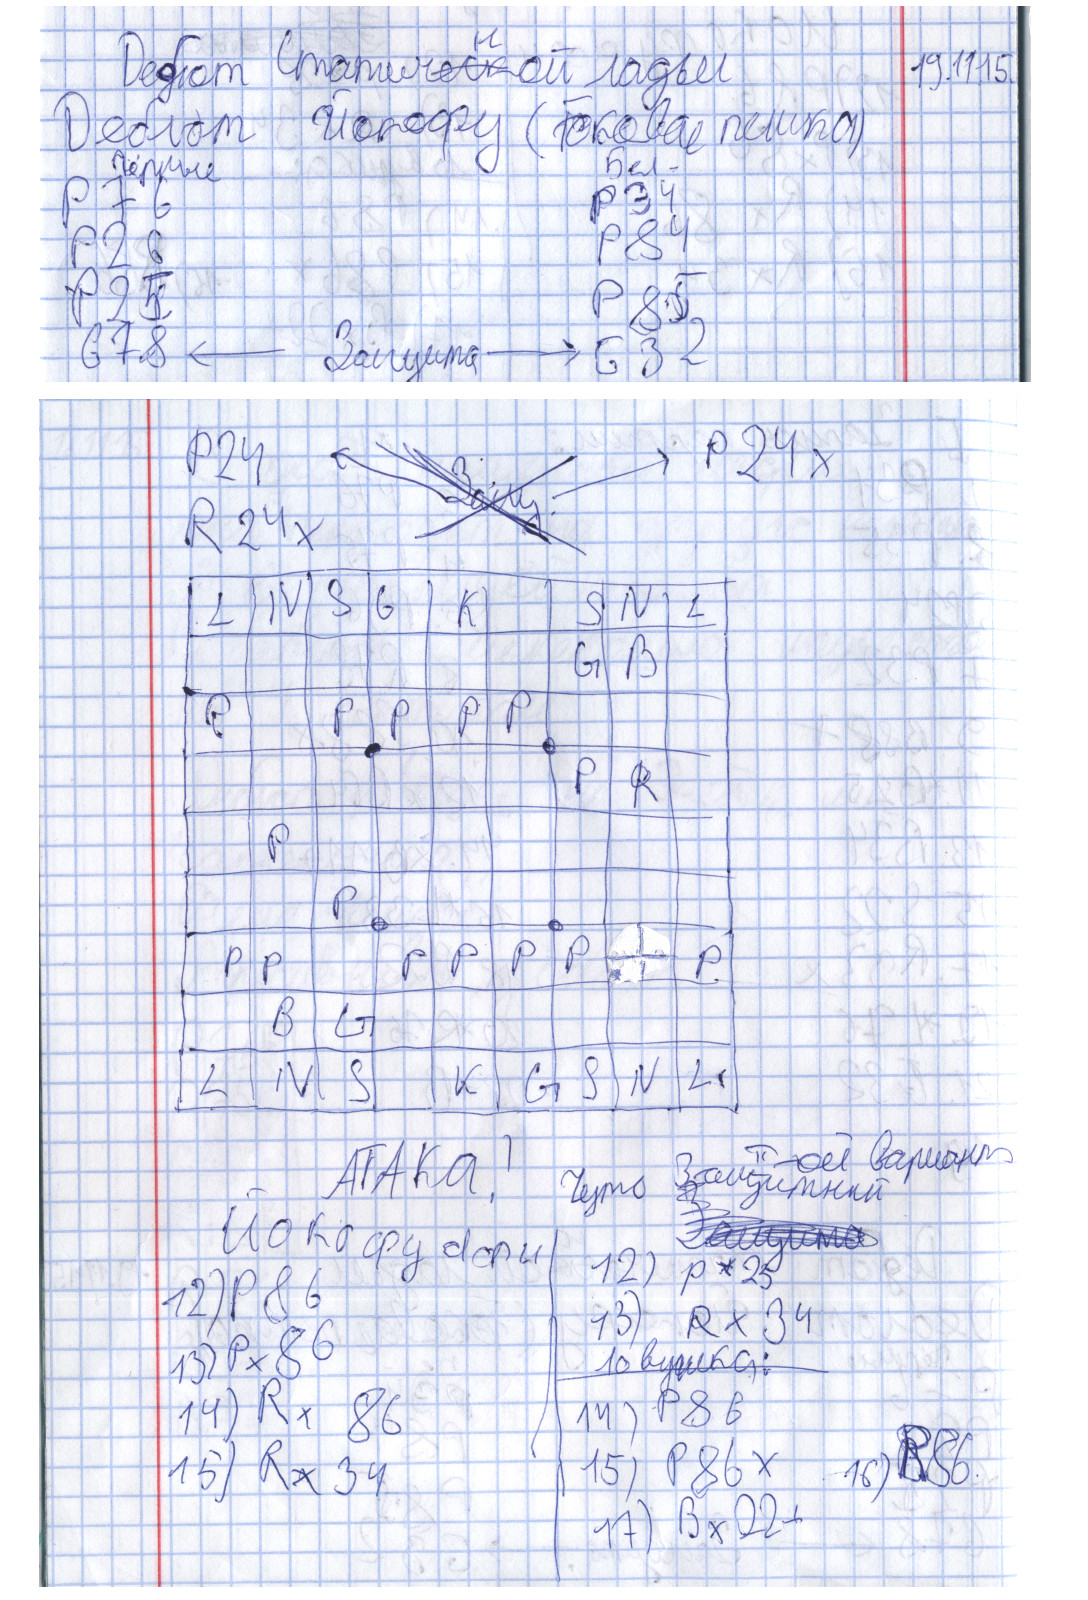
\includegraphics[scale=0.75]{suhomlin-total.jpg}\end{center}

Данный конспект написан Фёдором Сухомлиным.
К сожалению, конспектов подобного уровня в классе оказалось примерно три штуки.

\end{document}
